\section{Scientific considerations} % results consisting of comments of the reproducibility of the paper

\subsection{Reproducibility}
As seen in the checklist of the original paper no large efforts were made toward the reproducibility of the paper. For example, no links to working code or details on the fine-tuned model training were provided. This heavily impacted our work as we had to make many assumptions about the process. We did find, however, a repository at \href{https://github.com/yipei-wang/ClassContrastiveExplanations/}{https://github.com/yipei-wang/ClassContrastiveExplanations/} that contained some code regarding the fine-tuning of VGG-16 on CUB-200. This helped in specifying hyperparameters that would reflect those of the original paper. This also showed that they used VGG-16 with batch normalization, which was not specified in the original paper and the difference compared to the non-batch normalized variant will yield different results.

Lack of code or detailed method also led to difficulties reproducing some results, as seen in section \ref{experiments} especially coupled with some errors. For example, the inaccurate equation in section 5.1 in the original paper coupled with the wrong epsilon led to many difficulties in reproducing and understanding that section. It is also not specified as to which data the fine-tuned models are trained. There are also some minor mistakes such as the bird in Figure 1 of the original paper having the wrong input label.

We also found it unclear during our first readthroughs of the article that the authors' weighted contrastive method should ideally be implemented by back-propagating from the $p$ neuron and the performance gains that this gives. In general, the presentation of their weighted contrastive method as novel led us to miss the conclusion that it was proportional to back-propagating from the $p$ neuron for many explanation methods. Our experiments show, however, that for more sophisticated explanation methods more adjustments have to be made to the original method in order to make it contrastive by introducing negative areas.


\subsection{Scientific contribution}
The original paper provides an intuitive and efficient way of generating contrastive explanations that can take multiple classes into account. They also show that these outperform generally non-contrastive methods regarding the strength of the probability for the target class. They do not, however, make any large comparisons to state-of-the-art baselines in contrastive explanations. They defend this in peer reviews by claiming that many other contrastive methods ask the question of “how to change the instance to other classes?” while the authors aim to answer “why the instance is classified into this class, but not others?”. Furthermore, many other contrastive methods are only suitable for preliminary data such as MNIST rather than the high-resolution images used here. Therefore we deem this lack of comparisons to other methods as valid.

Another observation is that all results rely on the class probability $p$ as a metric for the relevance of the explainability method. While this is intuitive it also seems obvious that the contrastive weighted method presented which back-propagates from the $p_t$ neuron will outperform the same method based on the preceding $y_t$ neuron. This makes the results very expected, especially the ones shown in Figure \ref{f:grad_sign_perturbation_eps_003} and Table \ref{t:blurring}. The visualizations show, however, that this method yields a clear explanation as to which areas of the image are especially important for a certain class, and in the end, this is perhaps the greatest contribution. 

We also find that the authors' work is more of an explanatory nature than inventing something novel, as back-propagating from the $p$ neuron has been commonly done before and even mentioned in the original GradCAM paper \citep{gradcam}. The value is therefore showing that back-propagating from target softmax neuron $p_t$ yields a proven weighted contrastive explanation compared to back-propagating from logit $y_t$. 

\subsection{Dominating classes}
\label{dominate!!!}
The authors have explicitly chosen not to do experiments on images where there exist dominating classes where $p_1 \gg p_2$. This is not motivated in the paper but is likely because the contrastive weighted method tends to be reduced to the original, non-contrastive, explanation under such circumstances. This is easy to make note of during testing when looking at images where $p_2 \approx 0$ where the contrastive and non-contrastive versions show no qualitative difference. Table \ref{t:under_threshold} also shows a reproduction of Table \ref{t:blurring} but inverting the threshold and only using samples where the second most likely class has a probability $p_2 < 0.1$. This table clearly shows that the positive features between the original and weighted method are on average very similar while the negative regions in the weighted variant are slightly more effective in decreasing the target probability, although less so than in Table \ref{t:blurring}. 

That the explanation methods are so similar for low $p_2$ can be explained by $p_2$ often being very low, $< 0.001$, and much closer to $p_3$ than $p_1$. In those cases the weighted method when targetting the most likely class $t_1$ the subtracted weighted sum in Equation \ref{eq: weighted} will go toward zero as the non-target classes take out each other. As seen in Table \ref{t:under_threshold} this seems to mostly apply to the positive features of the weighted method and therefore it seems that the negative features of the non-target classes seem to be taking out each other.

Another reason for this behavior is explained by the observed relationship that explanation weights seem to increase with logit strength or output probability. This is exemplified in Figure \ref{fig:explanation-relationship}. Due to this, we can expect an explanation with regards to the dominating value to be weighted significantly higher, around 3 to 4 times, than all other features. For future work, normalizing the explanation before weighing could be considered.
\begin{figure}
    \tiny
    \centering
    % \resizebox{\textwidth}{!}{\
    % \begin{subfigure}{.48\textwidth}
    %     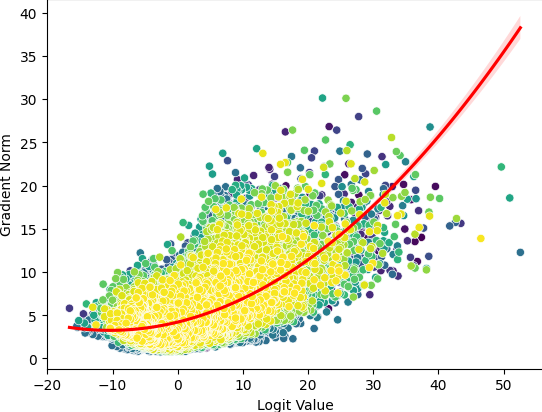
\includegraphics[width=0.97\textwidth]{figures/logit_gradientnorm_relationship.png}
    %     \caption{}
    %     % \caption{Relationship between the weighted and original explanation vectors depending on target prediction, $p_t$. A clear downwards trend can be observed.}
    %     \label{fig:explanation-relationship-topp}
    % \end{subfigure}
    % \hspace{0.5cm}
    % \begin{subfigure}{.48\textwidth}
    %     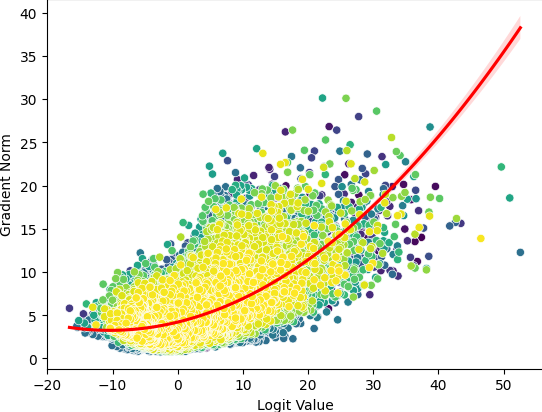
\includegraphics[width=0.97\textwidth]{figures/logit_gradientnorm_relationship.png}
    %     \caption{}
    %     % \caption{Relationship between the Explanation Vector and the logit strength, a clear upwards trend in explanation strength with logit can be observed.}
    %     \label{fig:explanation-relationship-logit-strength}
    % \end{subfigure}
    % }
    % caption{Relationship between the (a) top class prediction $p_t$ and the difference between the weighted and original explanation $\|\phi_p - \phi_y\|$ and (b) the relationship between the explanation weight $\|\phi_y\|$ and logit value $y$.}

    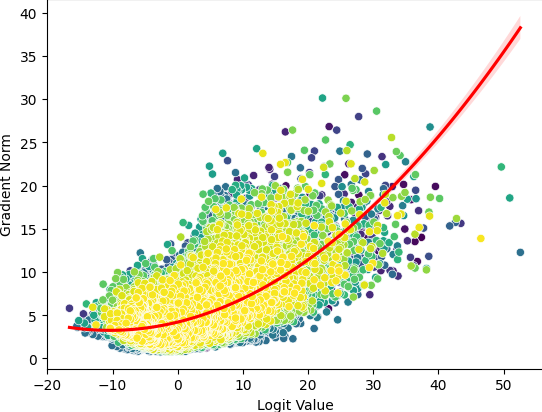
\includegraphics[width=0.47\textwidth]{figures/logit_gradientnorm_relationship.png}
    
    \caption{Relationship between the explanation weight $\|\phi_y\|$ and logit value $y$, using $\phi_y = \nabla_x y$ as an explanation, for 145 target classes for 1000 random images from ImageNet. A second-degree regression is applied and shows a clear upward trend (red). Colors are applied solely for visibility.}
    \label{fig:explanation-relationship}
\end{figure}

The behaviour of $\frac{\partial p_i}{\partial y_j}$ should also be considered. Here we observe that if the softmax output is dominated by a single value the gradient goes to zero. That if there exists a $p_t \to 1$ then it implicates $\frac{\partial p_i}{\partial y_j} \to 0$, this is easily observed in the Jacobian. 

One could also argue that there is no use of contrastive methods when there is only a single dominating class as then the model is certain in its decision and is not weigh the possibility of another class. However, in scenarios where a misclassification has occurred a contrastive method to compare the correct class to the misclassified class can be useful, thus there is a use for contrastive method even without dominating classes showing an opportunity for advancement in future work.

\begin{table}
    \tiny
    
    %\fontfamily{lmodern}\selectfont % Set font family to Latin Modern Sans Serif
    
    \centering
    \caption{Reproduction of Table \ref{t:blurring} using threshold criteria $p_2 < 0.1$ for GradCAM (GC). The probability of the second most likely class is almost always $p_2 \approx 0$ with an average $\bar{p}_2 = 0.01$, and has been omitted for this reason as it is mostly ambiguous.} \label{t:under_threshold}
    \vspace{2mm}
    \resizebox{\textwidth}{!}{\
    \begin{tabular}{c | c | c | c | c  c | c  c | c  c | c  c | c  c | c  c}
    %\abovetopsep
    \toprule
    %\hline
        \multicolumn{3}{c |}{} &
        \multirow{3}{*}{$p_t$} &
        \multicolumn{4}{c |}{Gaussian Blur} &
        \multicolumn{4}{c |}{Zeros} &
        \multicolumn{4}{c}{Channel-wise Mean} \\ \cline{5-16}

        \multicolumn{3}{c |}{} &
        &
        \multicolumn{2}{c |}{Pos. Features} &
        \multicolumn{2}{c |}{Neg. Features} &
        \multicolumn{2}{c |}{Pos. Features} &
        \multicolumn{2}{c |}{Neg. Features} &
        \multicolumn{2}{c |}{Pos. Features} &
        \multicolumn{2}{c}{Neg. Features} \\ \cline{5-16}

        \multicolumn{3}{c |}{} &
        &
        ori. &
        wtd. &
        ori. &
        wtd. &
        ori. &
        wtd. &
        ori. &
        wtd. &
        ori. &
        wtd. &
        ori. &
        wtd.\\

        \midrule

        \multirow{1}{*}{CUB-200} &
        \multirow{1}{*}{GC} &
        $t_1$ &
        0.985 &
        \textbf{0.981} &
        0.979 &
        0.442 &
        \textbf{0.351} &
        0.973 &
        \textbf{0.974} &
        0.438 &
        \textbf{0.358} &
        \textbf{0.977} &
        \textbf{0.977} &
        0.437 &
        \textbf{0.349} \\
    \midrule
    \end{tabular} }
\end{table}